% ---- tnf_paper.tex lines 1225-1288: The comparison at matched physical width ----
\section{The comparison at matched physical width}\label{sec:matchedwidth}

Two paragraphs above we disqualified a competitor on exactly the grounds this
section applies to ourselves. Tekum's widths count trits, so tekum16 is
$25.4$ bits and \emph{was never a 16-bit competitor at all}. The same sentence
is true of us. A TNF rung is named by its storage \emph{symbols} --- the
specification asserts $1 + E_t + M = N$ with $E_t$ counting trits --- so
``TNF16'' is one sign, four trits and eleven mantissa bits: sixteen cells and
\textbf{nineteen bits}. The gap widens along the ladder: $+2, +2, +3, +4, +5$
for TNF4, TNF8, TNF16, TNF32, TNF64.

That the naming sequence $4, 8, 16, 32, 64$ is exactly the IEEE width sequence
is what makes the error invisible. A row reading ``TNF16 against binary16''
looks matched and is not.

\begin{table}[t]\centering
\caption{Every rung against posit at its own \emph{physical} width, computed
from the committed reference implementations rather than quoted. ``Values'' counts
distinct non-zero decodings; ``step at $1.0$'' is the local relative gap between
neighbours, which bounds the rounding error in the working range.}
\label{tab:matchedwidth}
\begin{tabular}{llrrr}
\toprule
bits & format & values & binades & step at $1.0$ \\
\midrule
19 & TNF16 $(4t,11m)$ & $516{,}096$          & $127.0$ & $0.024\%$ \\
19 & posit19 $es{=}1$ & $\mathbf{524{,}286}$ & $68.0$  & $\mathbf{0.002\%}$ \\
19 & posit19 $es{=}2$ & $\mathbf{524{,}286}$ & $\mathbf{136.0}$ & $\mathbf{0.003\%}$ \\
19 & takum19          & $\mathbf{524{,}286}$ & $\mathbf{510.0}$ & $\mathbf{0.003\%}$ \\
\midrule
10 & TNF8 $(3t,4m)$   & $960$              & $31.0$ & $3.125\%$ \\
10 & posit10 $es{=}1$ & $\mathbf{1{,}022}$ & $32.0$ & $\mathbf{0.781\%}$ \\
10 & posit10 $es{=}2$ & $\mathbf{1{,}022}$ & $\mathbf{64.0}$ & $\mathbf{1.562\%}$ \\
\midrule
6  & TNF4 $(2t,1m)$   & $56$          & $14.6$ & $25.0\%$ \\
6  & posit6 $es{=}1$  & $\mathbf{62}$ & $16.0$ & $\mathbf{12.5\%}$ \\
6  & posit6 $es{=}2$  & $\mathbf{62}$ & $\mathbf{32.0}$ & $25.0\%$ \\
\bottomrule
\end{tabular}
\end{table}

\paragraph{The result is negative, and it is structural.} At every width the
ladder occupies, posit holds more representable values than TNF and a finer step
at unity --- by $12\times$ at 19 bits, $4\times$ at 10 and $2\times$ at 6. Worse
for us, posit with $es{=}2$ \emph{weakly dominates} TNF on both coordinates
simultaneously at all three: more binades \emph{and} a step no coarser. The
no-survivors corollary of \companion{the taper-catalogue section} does not survive being
restated at matched physical width, and is withdrawn to a matched-\emph{name}
claim.

The value deficit is not an encoding accident. A ternary exponent does not tile
a binary field: four trits need seven bits and use $81$ of $128$ codes, so
$8{,}190$ of the $2^{19}$ words are unreachable. No packing repairs this; it is
what a ternary exponent costs in a binary container.

\paragraph{What the negative result does not touch.} None of the above is a
cost figure, and the case for this format was never precision per bit. The
decoder cost, the multiplier removal and the zero-DSP result are measured on
standalone rigs that contain no exponent field comparison at all, and they are
unaffected. A format may lose every column of
Table~\ref{tab:matchedwidth} and still be the right choice where decode cost
dominates or where nothing else trains --- which is precisely the claim this
paper should be read as making.


% ---- tnf_paper.tex lines 1372-1427: Two width defects, and why they generalise ----
\section{Two width defects, and why they generalise}\label{sec:width}

\triptych{canon-tnf-12-width.png}{The two width defects of this section: a bus wide enough only for the configuration that was tested, the silent truncation this produced, and the clean sweep once every width is derived from the format's own parameters.}{fig:canon-width}


\companion{The hardware section} reports what the datapath costs once every bus is
derived from the format's own parameters. It was not measured that way first.
The two defects below --- one of area, one of correctness --- are the same
mistake, a width chosen by hand, and they are reported because that mistake is
not specific to TNF.

\subsection{Interface width dominated the arithmetic}
\triptych{canon-tnf-33-widthcost.png}{The bus was three times the width of the value it carried; once every width is derived from the format parameters the same arithmetic costs 219 LUTs and no DSP48 instead of 1,179 LUTs and three.}{fig:canon-widthcost}


Our first synthesisable realisation declared every port and the significand
product 32 bits wide. Nothing in TNF16 is 32 bits: the mantissa field was 9 at
the time of that build, so $1{+}M$ is 10 and their product is exactly 20; the exponent offset never exceeds
$\mathrm{OFFSET\_MAX}=80$, which is 7. Synthesis built a $32\times32$ multiplier
and a 32-bit comparison tree and charged for it (Figure~\ref{fig:width}):
1{,}179 LUTs, or three DSP48 blocks, against 219 LUTs and none once the buses
match the values they carry. The arithmetic is unchanged.

\begin{figure}[t]\centering
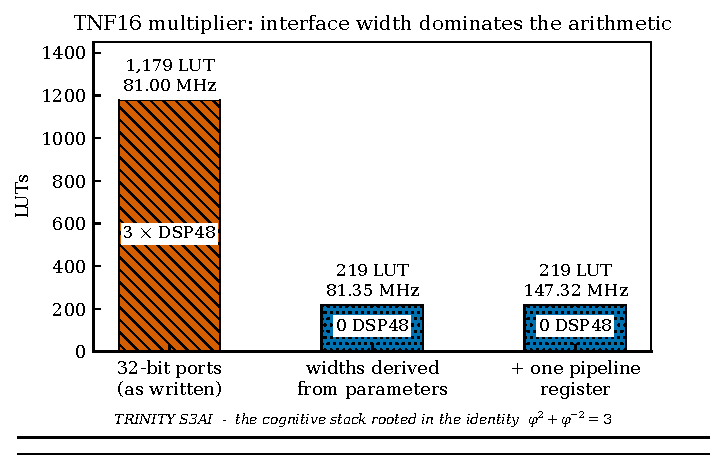
\includegraphics[width=\textwidth]{tnf_width.pdf}
\caption{The same arithmetic at three interface widths.}
\label{fig:width}
\end{figure}

\subsection{The same width decided correctness}
\triptych{canon-tnf-34-widthcorrect.png}{A 32-bit wire truncated a 52-bit significand product, and the failure was silent: 1,995,730 mismatches of 2,128,964 combinations against a 64-bit reference.}{fig:canon-widthcorrect}


At TNF32 the significand product needs 52 bits. The 32-bit wire truncates, and
the module returns wrong results while appearing to support the rung, since its
own documentation names TNF32 as a supported configuration. Measured against a
64-bit reference: 1{,}995{,}730 mismatches in 2{,}128{,}964 combinations.

Deriving every width from the format parameters removes both problems at once. We
report this because the pattern is not specific to TNF: in a parametric
arithmetic core, a width that is merely \emph{large enough for the configuration
that was tested} is a silent-truncation trap at the next one, and it will not be
caught by a testbench written against the tested configuration.


% ---- tnf_paper.tex lines 5721-6081: How a comparison fails while every measurement in it is correct ----
\section{How a comparison fails while every measurement in it is correct}
\label{sec:selfcheck}

Comparing number formats is harder than measuring them, and the two failures
are independent: nearly every difficulty encountered in this work left the
measurement intact and broke the comparison around it. The regularities below are
stated because they generalise past this subject, and because every quantitative
claim in this paper rests on having ruled them out. They are the conditions under
which a ratio between two formats means anything at all.

\paragraph{On what is being compared.} A ratio is meaningful only if both sides
were built as their own advocate would build them; seven times here a ratio
changed sign or magnitude when the other side was rebuilt
(\record{the scale-applier section}). Systems whose range scales differently with
width, one exact and one approximate, have no storage-matched ratio at all --- a
quantity depending on an unstated choice has no limit and cannot converge, which
is why six successive instrument corrections failed to settle one number. Where
one system's figure of merit is constant in a parameter and another's varies in
it, the well-posed comparison is a crossover and not a verdict
(the taper-delay theorem and \record{the crossover section}), and such a
crossover is an assertion about the workload rather than about the formats.

\paragraph{On the instrument.} Under placement-seed variation LUT count is
invariant and achieved frequency moves by $11.4\%$, so any metric combining them
inherits the timing variance in full, and a ranking resolves only rows separated
by more than that. A ratio over correlated factors restates the dominant one: on
the combined harness, ranking by throughput per area reproduced ranking by
$1/\text{area}$ at a Spearman correlation of $0.961$. And a result that moves the
same way under every successive correction is still moving.

\paragraph{On the harness.} Three defects appeared in the synthesis harness, none
visible in any number, each changing a headline by 10 to 50 percent; a second,
software harness contributed three more of its own, recorded in
\record{the applicability section}, so the total across both is six. A component shared by every
candidate is a confound rather than a constant, because it leaves area
differences intact and delay differences not. A harness observing part of a
design's output prunes each candidate in proportion to \emph{its own} output
width --- observing four bits of a 32-bit datapath left 27 LUTs of 179 while
leaving an adjacent 6-bit design nearly whole. And net-of-harness subtraction
requires the harness to be present in full in every build, since a design
consuming fewer of its sources prunes the rest.

\paragraph{On sources.} A defect found in an abstract is a hypothesis: abstracts
compress, and compression is indistinguishable from omission. An aggregated
search result may combine claims from several papers into wording present in
none. Both external criticisms we raised during this work dissolved on contact
with the papers themselves.


\paragraph{What this is worth.} Applied to two external papers read in full the
procedure produced no findings against them, and on both occasions caught our own
reading of them instead. We
therefore describe it as an instrument for checking one's own work, and not as a
method for auditing anyone else's. Three of the checks are mechanised as gates in
continuous integration; the full statement is in the accompanying note.





\subsection{Figures whose generating data is not in the repository}
\label{sec:provenance}
\triptych{canon-tnf-52-provenance.png}{The substring gate reports 882 of 885 distinctive literals as tracing to the tree; a stricter registry restricted to frequencies finds 16 of 40 with no record file, every one of them marked in place, and five document-to-code pairs still have no gate.}{fig:canon-provenance}

Twenty claims were withdrawn during this work, and a withdrawn claim's number
does not remove itself from a paper. A traceability check
(\texttt{tools/check\_paper\_numbers.py}) extracts every distinctive numeric
literal here and asks whether it appears in any file under \texttt{research/},
\texttt{fpga/} or \texttt{conformance/}. It excludes two classes rather than
tolerating them: constants stated beside the formula that produces them ($23$ of
them, correctly absent from any data file), and rounding, where a data literal
extending the printed digits counts as the source.

Re-run on this revision over $6{,}108$ data files, the check reports $885$
distinctive literals of which two trace to no file. That figure is an artefact of
how the check matches, and the honest number is larger.

The weakness was found by auditing the check's passes rather than its failures. It
matches a literal as a \emph{substring} of a data file's text with separators
stripped, so a short literal is reported as sourced whenever its digits occur
inside a longer unrelated number. Two figures reading $3.15$ passed on exactly that
basis and neither had a generating file: a takum32 decode table in Mbit, now
withdrawn from \record{the zero-path corollary}, and the octave span of
\record{the barrel-range theorem}. A frequency such as $307.69$ passes because the
digits $30769$ appear inside a conformance-vector column. A literal of three or
four significant characters should be matched on word boundaries; until the gate
does so, its pass is weak evidence for short literals and no evidence at all for
frequencies.

A second, stricter registry (\texttt{tools/}\allowbreak\texttt{freq\_provenance.py},
output in \texttt{research/}\allowbreak\texttt{arxiv\_tnf/}\allowbreak\texttt{freq\_provenance.json}) was therefore written for the
one quantity in this paper with the widest seed spread: achieved frequency. It
takes only prose and script files --- \texttt{*.md} and \texttt{*.py} under
\texttt{research/}, \texttt{fpga/}, \texttt{conformance/}, \texttt{docs/} and the
repository root, the places where a measurement is actually written down --- and it
requires a delimited match rather than a substring. Its result on this revision:
of \textbf{40} frequency literals in this paper, \textbf{16} are stated in no
record file. Every one of the sixteen is marked $^{\ast}$ where it appears, and
carries no hardware-performance claim.

The distribution of the sixteen is the part that matters. All fifteen marked rows
of \record{the full-throughput table} are baselines or formats whose frequency was
never written down; the six unmarked rows are all ours. The same asymmetry holds in
\record{the T-Net table}, where all three posit frequencies are unsourced and all three
TNF frequencies trace to
\texttt{TNF\_SPEC\_CORRECTION\_2026-08-11.md} or
\texttt{BROKEN\_IS\_SMALL\_2026-08-11.md}. An ordering by MHz per LUT in which our
rows have records and the rows they are ranked above do not is not evidence of the
ordering, and is presented here as illustrative.

Worse, and decisive for the release question: \textbf{no place-and-route log behind
any frequency quoted in this paper is in the repository tree}. At commit \texttt{a0fb006}, \texttt{git ls-files} finds five \texttt{*.log} files, all under \texttt{measurements/pnr\_logs/} and all five seeds of one design (\texttt{e2m11\_add}) that no frequency here is sourced to; beyond those, the only log in the working tree is the \LaTeX{} log of this document. The note \texttt{research/frontier/WITHDRAWAL\_FMAX\_UNSOURCED\_2026-08-10.md}, which retracts itself in its own heading, states that the ladder frequencies
rest on $298$ \texttt{nextpnr-xilinx} logs under \texttt{fpga/phiscale/}; that
directory holds $163$ files at the same commit and none of them is a log. So even the twenty-four
sourced frequencies are sourced to a \emph{document that reports a measurement},
not to the tool output that produced it. Under the standard this paper applies
elsewhere --- a claim is closed by a command, its inputs, its log and a hash --- the
entire frequency column of this paper is open. It is reported, marked, and not
relied upon for any conclusion.

One further disagreement belongs here rather than in a footnote. The same
twenty-one-point experiment is tabulated twice in this project: as
\record{the full-throughput table} here, and in \texttt{fpga/tnet/MATRIX.md}, which
describes itself in the same words --- one synthesised datapath, XC7A200T, no DSP,
one harness. The two disagree row by row. \texttt{binary16} reads $552$ LUT at
$62.69$ there against $522$ at $63.30$ here; takum16 $817$ at $64.16$ against $789$
at $58.96$; GFTernary $466$ at $82.51$ against $463$ at $83.19$; posit32 $955$ at
$28.33$ against $953$ at $28.16$; the 16-bit TNF rung $495$ at $71.90$ against $565$
at $66.28$. Two tables for one described experiment is exactly the document-to-code
pair Theorem~\ref{thm:doctrace} below predicts will go unguarded, and it is not
resolved by choosing the more favourable one. Until a run reconciles them, neither
is the record.

\begin{table}[t]\centering
\caption{Figures with no record file in the repository, on this revision, from the
strict registry. Table and theorem names in the middle column refer to
\recordname, where the full twenty-one-row experiment is tabulated. Each figure
is retained and marked $^{\ast}$ at every point of use, and
none supports a hardware-performance claim. Earlier revisions of this subsection
reported two or three such figures; that count came from the substring gate and is
restated here rather than carried forward. The octave span was found by auditing
the gate's passes and is not a frequency.}
\label{tab:untraced}
\begin{tabular}{lll}
\toprule
figure & where it appears & class \\
\midrule
$318.47$\,MHz & plastic 16-bit, hierarchy table & ours, unsourced \\
$83.19$\,MHz & GFTernary, full-throughput table and text & ours, unsourced \\
$78.83$\,MHz & \texttt{int8}, rejected-format table and text & baseline \\
$77.00$\,MHz & \texttt{binary32}, full-throughput table & baseline \\
$73.51$\,MHz & VAX F, full-throughput table & baseline \\
$72.16$\,MHz & GF10, full-throughput table & ours, unsourced \\
$71.15$\,MHz & GF14, full-throughput table & ours, unsourced \\
$67.06$\,MHz & fp8 e5m2 and minifloat, full-throughput table & baseline \\
$67.02$\,MHz & fp8 e4m3, full-throughput table & baseline \\
$63.30$\,MHz & \texttt{binary16}, full-throughput table & baseline \\
$58.96$\,MHz & takum16, full-throughput table & baseline \\
$46.78$\,MHz & IBM hex32, full-throughput table & baseline \\
$44.33$\,MHz & posit8, T-Net table and full-throughput table & baseline \\
$43.04$\,MHz & LNS16, full-throughput table & baseline \\
$40.38$\,MHz & posit16, T-Net table and full-throughput table & baseline \\
$28.16$\,MHz & posit32, T-Net table and full-throughput table & baseline \\
\addlinespace
$3.15$ octaves & 210-layer scale range, barrel-range theorem & not a frequency \\
\bottomrule
\end{tabular}
\end{table}

Neither check can show a number is right; they find numbers with no source, which
is strictly weaker and still enough. A figure nobody can trace to a file is one
nobody can re-check, and after twenty withdrawals that is exactly where a stale
value survives. Sixteen of the seventeen entries above are achieved frequencies,
the quantity with the widest seed spread in this paper, and none of them should be
quoted without a re-measurement whose log is committed. The remaining entry was
found by the substring audit rather than by either gate, and the two-bit shift
field that \record{the barrel-range theorem} concludes from it survives any span below
four octaves, so that conclusion is more robust than the figure supporting it.

What this subsection therefore does not claim: that the frequency measurements are
wrong. They may well be right. It claims that at this revision they are not
reproducible from the released artefact, that this is a defect of the artefact and
not of the design, and that the way to close it is a place-and-route run whose
constraints, tool versions, seed, timing report and worst slack are committed
alongside the numbers --- not a further edit to this paragraph.

\begin{theorem}[A document is an artefact, and its pairs need guarding]
\label{thm:doctrace}
Consistency checks are written between artefacts that a tool already reads
together --- compiler, simulator, build script. Documents are read only by
people, so every pair involving one goes unchecked by construction, and that is
where withdrawn numbers persist.
\end{theorem}

Enumerating the pairs is what makes a search for such defects systematic rather
than accidental. Three earlier gates in this work were each found by tripping
over the defect they now catch, and all three guard code against code.
Enumerating every pair that must agree exposed five unguarded ones in a single
pass, all of them with a document on one side.



\subsection{The staircase form prescribes the comparison}
\triptych{canon-tnf-53-staircasecmp.png}{The staircase form decides whether a comparison needs a line, an exponential crossover or a duty cycle, and for a periodic wobble the honest report is 50/50.}{fig:canon-staircasecmp}

\label{sec:formprescribes}

\companion{The taper-catalogue section} classifies tapers by staircase form to \emph{describe}
them. Measuring the crossovers of \record{the crossover section} over two fitting
windows shows the classification does more than that.

\begin{theorem}[The staircase form decides whether a window is needed]
\label{thm:formwindow}
A crossover between a fixed field and a taper depends on the fitting window if
and only if the taper's staircase form is not arithmetic. An arithmetic taper's
$M_{\mathrm{eff}}$ is linear in $|e|$, so its slope is well-defined without a
window. A geometric taper's is linear in $\log|e|$, so no line fits it and its
apparent slope is a property of the window alone.
\end{theorem}
\begin{proof}
Write the fixed-field comparison as $m=M_0$ and the taper as $M(e)$.
For an arithmetic taper, $M(e)=a-c|e|$ on each branch, so solving
$M(e)=m$ gives a linear binade coordinate independent of the chosen fitting
window.  For a geometric taper, $M(e)=p-\log_2|e|$; a line fitted over
a window replaces this logarithm by a window-dependent surrogate slope.
Changing the window therefore changes the inferred crossing, whereas the
closed logarithmic equation does not.  Thus window dependence is equivalent
to the failure of the arithmetic form in the stated model.
\end{proof}

Measured across windows $1$--$9$ and $1$--$20$, the split is exact: posit16,
posit32 and posit64 move by $1.08\times$, $1.00\times$ and $1.09\times$, while
every takum rung --- including the takum-layout oracles formerly labelled
tekum --- moves by $1.39\times$ to $1.72\times$.

\begin{corollary}[Closed form for a geometric taper]
\label{cor:geomcross}
For a geometric taper, $M(e) = p - \log_2 e$, so the crossover against a fixed
field of constant $m$ solves exactly:
\[
  x = 2^{\,p-m},
\]
with no window required.
\end{corollary}
\begin{proof}
At the crossing, equality with the fixed field gives
$p-\log_2 x=m$.  Rearranging yields $\log_2 x=p-m$ and hence
$x=2^{p-m}$.  The equation contains no fitting-window endpoints, so the
closed crossing is determined by the two model parameters alone.
\end{proof}

\begin{table}[t]\centering
\caption{Crossovers, computed by the model each taper's form requires. A
straight-line fit had overstated every geometric taper's reach, because a line
under-reports how fast a logarithm falls near the origin.}
\label{tab:crosscorrected}
\begin{tabular}{llr}
\toprule
taper & form & crossover, binades \\
\midrule
posit8 & arithmetic & $1.5$--$2.5$ \\
posit16 & arithmetic & $8.5$ \\
posit32 & arithmetic & $9.2$ \\
posit64 & arithmetic & $54.0$ \\
takum16 & geometric & $\mathbf{1.8}$ \\
takum32 & geometric & $\mathbf{2.6}$ \\
takum64 & geometric & $\mathbf{62.7}$ \\
takum-layout ``tekum16'' oracle & geometric & $\mathbf{2.1}$ \\
takum-layout ``tekum32'' oracle & geometric & $\mathbf{2.4}$ \\
takum8, takum-layout ``tekum8'' & geometric & TNF everywhere \\
\bottomrule
\end{tabular}
\end{table}

Six figures previously reported as ranges were computed by the wrong model and
are corrected here: takum32 moves from $5.9$--$10.2$ to an exact $2.6$, the
takum-layout ``tekum16'' oracle
from $4.2$--$6.5$ to $2.1$. (True tekum, arXiv:2512.10964, counts its width in
trits and has no 16-bit member.) The remaining window dependence is confined to
posit8, whose peak sits within $0.45$ bits of TNF8's so that any slope estimate
divides a very small number.

The point worth keeping is not the arithmetic. \textbf{A taxonomy introduced to label
formats turns out to prescribe how they must be compared} --- arithmetic tapers
by a linear crossover, geometric ones by $2^{p-m}$. A classification that only
labelled would not do this, and we had used it only to label for most of this
work.



\begin{theorem}[A wobble admits no crossover]
\label{thm:wobblecross}
If a format's $M_{\mathrm{eff}}$ is periodic in $|e|$ with amplitude $A$ and
period $P$, and a constant-form competitor's $m$ lies strictly inside the band,
then no $x$ exists such that one leads for all $|e| < x$ and the other for all
$|e| > x$. The well-posed statistic is the duty cycle --- the fraction of each
period on which each leads --- together with $P$.
\end{theorem}
\begin{proof}
Because $m$ lies strictly inside the attained band, one phase in every period
has $M_{\mathrm{eff}}>m$ and another has $M_{\mathrm{eff}}<m$. Periodicity
repeats both phases after every integer multiple of $P$, arbitrarily far along
the $|e|$ axis. Therefore neither ordering can hold on a whole tail
$|e|>x$, so a single crossover point does not exist. The fraction of one
period occupied by the set $\{e:M_{\mathrm{eff}}(e)>m\}$ is invariant under
translation by $P$; its complement is the opposing duty cycle. Recording that
fraction together with $P$ therefore captures the repeated comparison without
inventing a nonexistent threshold.
\end{proof}

Measured on IBM hexadecimal 32, whose $M_{\mathrm{eff}}$ by binade reads
$21.03$, $21.75$, $22.94$, $19.95$, then repeats: amplitude $3.07$ bits, period
$4$ binades, which is $\log_2 16$ as the radix requires. Against packed TNF32 at
$M_{\mathrm{eff}} = 21.32$, inside the band $[19.94, 23.11]$, the winner
alternates with that period at a duty cycle of $50/50$, and no binade separates
them.

\begin{corollary}[The taxonomy is prescriptive]
\label{cor:taxprescribes}
Each of the four staircase forms determines the \emph{shape} of a well-posed
comparison against a constant format: a difference for constant, a linear
crossover for arithmetic, an exponential crossover $2^{p-m}$ for geometric, and a
duty cycle for wobble.
\end{corollary}
\begin{proof}
For the constant form, subtracting the competitor leaves a constant difference,
so there is no crossing coordinate to solve for.  The arithmetic form is linear
in $|e|$, giving the linear crossing in Theorem~\ref{thm:formwindow}; the
geometric form gives $x=2^{p-m}$ by Corollary~\ref{cor:geomcross}.  For a
periodic wobble, Theorem~\ref{thm:wobblecross} rules out a single crossing and
leaves the duty cycle as the well-posed statistic.  These four cases exhaust the
staircase forms used by the taxonomy, so the prescribed comparison shape follows.
\end{proof}

The mapping from form to answer-shape is stated here, and we make no claim about
how the literature reports. An earlier version of this paragraph said that
published comparisons give verdicts or ratios; checked against Hunhold's takum
paper, that is false --- it reports by regime with numeric thresholds, noting
that posit's efficiency ``markedly diminishes with deviation from unity'' and
that takum's accuracy ``exceeds that of posits near unity, nearly aligning with
it for slightly larger exponents.'' The sentence is withdrawn.

What we have not found in that literature is the closed form $2^{p-m}$ for a
geometric taper against a constant-form competitor, or any treatment of the
wobble case. The contribution here is the mapping itself: the form of the answer
is fixed by the competitor's staircase, and a classification introduced only to
label formats turns out to settle it.
\triptych{canon-tnf-72-correctedcrossov.png}{The section replaces six line-fit crossover ranges with form-appropriate values and withdraws an inaccurate characterisation of the published takum comparison.}{fig:canon-b4-72correctedcrossov}




% ---- tnf_paper.tex lines 6082-6194: Adjacent work this paper is measured against ----
\section{Adjacent work this paper is measured against}\label{sec:adjacent}

Four bodies of work published while this paper was being prepared bound its
claims, and each is named here rather than left to a reader to supply.

\paragraph{The standards baseline.} The binary baselines used throughout ---
\texttt{binary16}, \texttt{binary32}, \texttt{binary64} --- are the ones defined
by IEEE Std 754-2019~\cite{ieee754_2019}, and the eight- and four-bit baselines
are the ones being fixed by the IEEE P3109 working
group~\cite{p3109wg2026}. The 83-format catalogue this work draws its
conformance vectors from cross-walks against P3109 explicitly~\cite{catalogue}.

\paragraph{Two independent machine-checked treatments of the nearest standard.}
P3109 arithmetic has been formalised twice and independently: in Imandra/IML,
presented at ARITH 2025~\cite{wintersteiger2025}, and in Lean, as
FLoPS~\cite{flops2026}. This bounds the claim this paper makes about
auditability. Bit-exact conformance vectors establish determinism of a decode
and arithmetic law against an independent oracle; when the same vectors are
replayed on a board, and the bitstream fingerprint, the device identifier and the
transcript are archived together, they establish determinism \emph{on that part}.
A mechanised proof establishes semantics instead. These are different layers, and
this work supplies conformance in the reported open flow, not a mechanised
semantics. The gap between those layers is narrowing and it should be said so:
formally verified \emph{synthesizable} floating-point data types have now been
demonstrated inside an HDL~\cite{archhdl2026}, which moves machine-checked
guarantees from the model down to the register-transfer description that gets
synthesised, and the broader formal-verification effort for floating-point
arithmetic continues independently of the P3109 track~\cite{mohanty2025}, while
the cost of applying formal tools to register-transfer code is itself falling, with
open-source multi-agent pipelines now reported for formally checked RTL
repair~\cite{tran2026rtlrepair}, and an executable hardware-intent layer has been
proposed to make microarchitectural obligations explicit before RTL lowering
and synthesis~\cite{cheng2026hint}. Against
that, a conformance transcript replayed on a specific part is not a weaker proof
of the same thing but a different object: it is evidence about a physical device
and its bitstream, which a proof about an HDL description does not provide, and it
is silent about semantics, which the proof does provide. This paper claims only
the former. The same line of
work also supplies $\kappa$-approximation~\cite{fitzgibbon2026kappa}, a
scale-invariant accuracy measure on the standards track; the error figures
reported here are mean relative error over exact rationals and are not
$\kappa$-approximation figures, and should not be read as such.

\paragraph{Bit-exactness as an audit primitive.} The use this paper makes of
conformance vectors --- a reproducible fingerprint of an arithmetic law --- is the
same primitive being developed for inference auditing, where bitwise-precise
re-computation is shown to be achievable without a performance
penalty~\cite{cankaya2026}. That line supports the value of the primitive and
must not be conflated with a different sense of determinism, obtained by
scheduling and verified speculation over arithmetic that is itself not
bit-reproducible~\cite{gond2026llm42}. The two are separate layers, and only the
first is what a format can supply. The distinction is not academic: a 2026 study
locates the numerical instability of large-model inference in the arithmetic and
the reduction order rather than in the schedule, and has to intervene at that
level to obtain reproducible output~\cite{zhu2026heal}, which is evidence that the
layer a format governs is the binding one. The first layer is also acquiring load-bearing
applications rather than only audit arguments: byte-exact reuse of cached
intermediate state across models has been used as the correctness condition of a
knowledge-transfer pipeline~\cite{schelpe2026grafting}, where a single differing
byte invalidates the construction. Whatever one makes of the pipeline, it is an
instance of bit-exactness being consumed as a contract rather than reported as a
virtue, which is the direction that makes a conformance ledger worth publishing.

\paragraph{Earlier combinations of tapering and a non-standard radix.} The
tapered-precision route is older and wider than the posit and takum line cited
above: a tapered floating-point extension has been proposed for the redundant
signed radix-2 system via canonical recoding~\cite{schoenbaum2021}, which is a
prior combination of tapering with a non-standard digit set and is acknowledged
here as such. The takum line has meanwhile been evaluated outside machine
learning, in sparse linear solvers against bfloat16 and posit~\cite{hunhold2024sparse},
which is the closest thing available to an independent accuracy baseline for
tapered formats and is the reason no accuracy superiority over takum is claimed
in this paper.

\paragraph{Accuracy is not a property of the field layout alone.} Matsuoka's
two-part argument~\cite{matsuoka2026fp8a,matsuoka2026fp8b} separates
\emph{precision} --- the native width of the format --- from \emph{accuracy},
recovered by the accumulation strategy, with Kulisch fixed-point accumulation as
the escape route. That separation supports the position taken here that the
$\varphi$ rule is a rule for choosing fields and not a different arithmetic, and
it also limits it: no field layout at sixteen bits removes the need for a wider
accumulator. The comparative picture across INT and FP at fine granularity is
surveyed for the same generation of formats in~\cite{int_vs_fp2025}, and the
performance--efficiency trade-off for low-precision formats was mapped
earlier in~\cite{mlformats}.

\paragraph{A direct threat to the representation--computation separation.}
CurveFP is a recent and materially different warning against over-generalising
the separation used in this paper: it co-designs a block-scaled,
logarithmic representation with a closed product operation, and reports
downstream language-model results together with a preliminary accelerator-tile
area result~\cite{qiao2026curvefp}. We therefore mark it as
\textbf{[threat]} to any claim that a representation-level observation is
unlikely to transfer to computation. It is not a head-to-head comparison with
TNF: CurveFP uses block scales and interleaved logarithmic curves, whereas TNF
uses a fixed ternary-derived field split, and the result record is a preprint
with a different workload and hardware model. The conclusion supported here is
narrower: our own TNF evidence must be stated as task- and rung-specific, and
the conjugate-gradient table above is not evidence about language-model
training, product closure, area, or energy. A direct CurveFP--TNF experiment
remains open.

\paragraph{Contemporaneous ternary and alternative-format hardware.} Ternary
inference hardware on FPGA is an active line independent of this
one~\cite{tereffic2025,tenet2025}, although it ternarises \emph{weights} rather
than the number representation. Posit arithmetic has been evaluated on FPGA and
GPU accelerators with quantified logic overhead~\cite{posit_accel2024}, and
logarithmic number systems have been co-designed with LLM datapaths on
FPGA~\cite{pnnl_lns2025}; both are baselines in the tables above. Uses of the
golden ratio in computing have been surveyed
systematically~\cite{akhtaruzzaman2024phi}, and the present rule should be read
against that survey rather than as an isolated idea.


% ---- tnf_paper.tex lines 6195-6271: What the formal statements are, and what they are ----
\section{What the formal statements are, and what they are
not}\label{sec:statusofstatements}

This paper carries a large number of numbered statements, and they are not all the
same kind of object. Collecting the distinction in one place is a service to a
reader who wants to know which lines could be wrong for a mathematical reason and
which could be wrong for an empirical one.

\paragraph{Three kinds of statement.} The first kind is \emph{analytically
proved}: it follows from arithmetic, from the irrationality of $\log_2 3$ or
$\varphi$, or from an algebraic identity, and no measurement can disturb it.
The economy, no-free-lunch, packing-density and Lucas-trace theorems of
\companionname, and the $\varphi$-rounding-envelope lemma, the
$\varphi$-ratio bound and the negative-product proposition of \recordname,
are of this kind. The second kind is a
\emph{proposition about a model}: it is a correct deduction from a cost model,
error model or workload assumption that is itself an idealisation, so it is exactly
as reliable as the model it is stated over --- the $\kappa$ statements and the
width-rule optimisations belong here, and the way for them to fail is for the
model to be the wrong model, not for the algebra to be wrong. The third kind is an
\emph{empirical observation} stated in numbered form for reference: post-route
resource and frequency figures, perplexity comparisons, and error measurements
over sampled distributions. These can be falsified by rerunning them, and the
places where our own earlier runs were falsified in exactly this way are recorded
in Section~\ref{sec:limitations-anchor} and in the erratum discussion.

\paragraph{Eight conclusions this work supports.} The following are the load-bearing
conclusions, each with the status it actually has.

\begin{enumerate}
\item The $\varphi$ split has a \emph{finite-width} certificate and not only an
asymptotic one: for $e\geq1$ the deviation of $m/e$ from $\varphi$ is strictly
below $\varphi^{2}/(2e)$ (\record{the $\varphi$-ratio bound}). The residual can
therefore be reported at a given width rather than promised in a limit
[proved].

\item The exact coefficient $\varphi^{-2}$ never produces an ambiguous rounding at
any non-zero width (\record{the $\varphi$-rounding-envelope lemma}); every tie-breaking
ambiguity in circulation comes from a truncated decimal surrogate for the
coefficient, and first bites at $N=12{,}239$ [proved].

\item Packing a ternary exponent into bits is not merely lossy: the count of
unreachable codes is positive and odd at every trit budget, and the utilisation
visits a dense subset of $(1/2,1)$, so no tail of the ladder is asymptotically
efficient (\companion{the packing-density theorem}) [proved].

\item Even powers of $\varphi$ admit an integer-only certificate through
$S_{n+2}=3S_{n+1}-S_n$ (\companion{the Lucas-trace theorem}), which makes a depth-$k$
$\varphi$-stack auditable with no rounding model in the loop. This is a testability
result, not an accuracy claim [proved].

\item One additional ternary exponent position multiplies the scale-state count by
three and halves the significand cell count. That exchange rate is exact and it is
the whole content of the static split [proved].

\item Objectives of the form $R^{a}P^{b}$ never select an interior split
(\record{the negative-product proposition}). The $\varphi$ rule therefore cannot
honestly be presented as the maximiser of a range-times-precision product, and
this paper does not present it as one [proved --- negative result].

\item The new ratio bound was additionally checked by exhaustive integer
enumeration at every $N=4,\dots,100{,}000$ with no violation. This is a
sanity-check on the proof, not a substitute for it [measured].

\item An objective that could justify the $\varphi$ split for a specific workload
would have to carry the value distribution, the overflow policy and a hardware
cost model. No such objective is derived here, and constructing one is left open
[open].
\end{enumerate}

\paragraph{Two facts that constrain rather than support the design.} Etiemble's
argument that three is not the optimal radix for computation~\cite{etiemble2019} is
accepted here on its own terms, and the microscaling study showing that finer
granularity is not monotonically better~\cite{fasoli2026} bounds how far any
scale-grid refinement can be expected to go. Both are cited above at the points
they bear on, and neither is treated as a matter of opinion.


% ---- tnf_paper.tex lines 6272-6734: Three results added in this revision, one of which weakens a claim ----
\section{Three results added in this revision, one of which weakens a claim}\label{sec:threeresults}

This revision adds three results that were open in the previous one. The order is
deliberate: the first fixes the reference artefact, the second turns the format
question into a solved optimisation and in doing so \emph{withdraws} an advantage
the earlier framing granted us, and the third settles a question about the
golden-ratio datapath with a measurement rather than an appeal.

\subsection{The reference oracle is now versioned, not corrected}
\label{sec:variantA}

Limitations item~7 in the previous revision recorded that the shipped
\texttt{tnf\_ref.py} ladder sat on research-note widths and that some rungs failed
the width rule $1 + E_t + M = N$. The count in that item was wrong in our favour:
it said three, and an audit of all nine rungs says \textbf{seven}.
Table~\ref{tab:ladderversions} lists them.

\begin{table}[t]\centering
\caption{Every rung of the shipped oracle against the width rule
$M = N - 1 - E_t$. Seven of nine violate it. The v2 column is the
specification of \companion{the specification table}; v1 is kept, not deleted, because published
figures were computed at those widths.}
\label{tab:ladderversions}
\begin{tabular}{lrrrrr}
\toprule
rung & \multicolumn{2}{c}{v1 research note} & $1{+}E_t{+}M$ & \multicolumn{2}{c}{v2 specification} \\
\cmidrule(lr){2-3}\cmidrule(lr){5-6}
 & $E_t$ & $M$ & & $E_t$ & $M$ \\
\midrule
TNF4    & 2 & 1    & 4 \checkmark   & 2 & 1    \\
TNF8    & 3 & 4    & 8 \checkmark   & 3 & 4    \\
TNF16   & 4 & 9    & 14 $\times$   & 4 & 11   \\
TNF32   & 5 & 21   & 27 $\times$   & 6 & 25   \\
TNF64   & 7 & 52   & 60 $\times$   & 7 & 56   \\
TNF128  & 8 & 115  & 124 $\times$  & 8 & 119  \\
TNF256  & 9 & 242  & 252 $\times$  & 9 & 246  \\
TNF512  & 10 & 497 & 508 $\times$  & 10 & 501 \\
TNF1024 & 11 & 1006 & 1018 $\times$ & 11 & 1012 \\
\bottomrule
\end{tabular}
\end{table}

The repair is not a patch. Both ladders now ship as named ladder versions,
\texttt{v1-research} and \texttt{v2-spec}, and every conformance vector carries
that name in its filename and in its own header, beside the vector specification
version --- \texttt{tnf-vectors-2} when this repair was made --- which also names
the SHA-256 manifest that pins the digest of every file in the set. A figure
computed at v1 stays reproducible at v1; a specification claim is checked against
v2. Eighteen vector files per specification version, 1{,}038 rows each, were
generated from a self-contained \textsc{splitmix64} stream rather than
the language's own generator --- a standard-library PRNG is an implementation
detail and not a contract --- with the per-rung seed derived by hashing
\texttt{version|width|trits|mantissa|op}, so adding a tenth rung cannot shift the
stream of an existing one. Regeneration reproduces the manifest of the current
specification version byte for byte; that version string is hashed into every
per-rung seed, so a superseded set stands on the digests recorded for it rather
than on re-execution.

The oracle also gained the check whose absence produced the sign defect. Add/mul
commutativity is blind to an inverted sign, because the inversion survives on both
sides of $a+b=b+a$; a round-trip assertion is not. Both ladders now pass 72
round-trip probes and the commutativity suite at all nine rungs with zero
violations \textbf{[proved]}.

\subsection{The format question is a solved optimisation, and the answer stops favouring us}
\label{sec:variantB}

\begin{theorem}[The ternary exponent buys no range per stored bit]
\label{thm:rangeperbit}
Let $t \ge 1$ be a trit budget and let $b = \lceil t\log_2 3\rceil$ be the number
of binary storage cells that field occupies. The ternary field addresses $3^t$
codes, hence $3^t - 1$ binade steps; a binary field of the same $b$ cells
addresses $2^b$ codes, hence $2^b - 1$ steps, of which $2^b - 2$ remain after
reserving one code for the non-finite class. Then
\[
2^b - 2 \;\ge\; 3^t - 1,
\]
with equality if and only if $t = 1$.
\end{theorem}

\begin{proof}
By definition of the ceiling, $2^b \ge 3^t$. Suppose $2^b = 3^t$ for some
$t \ge 1$; then $2 \mid 3^t$, which is false. Hence $2^b > 3^t$, and since both
sides are integers, $2^b \ge 3^t + 1$, i.e.\ $2^b - 2 \ge 3^t - 1$. For $t = 1$:
$b = 2$, $2^b - 2 = 2 = 3^1 - 1$, equality. For the converse, suppose equality
holds, i.e.\ $2^b - 3^t = 1$, so $2^b - 1 = 3^t$. If $b$ were odd then
$2^b \equiv 2 \pmod 3$ and $2^b - 1 \equiv 1 \pmod 3$, so $3 \nmid 2^{b}-1$, while
$3 \mid 3^{t}$ for every $t \ge 1$; the case $t = 0$ is excluded by hypothesis. Hence $b = 2c$ is even and
\[
  (2^{c}-1)(2^{c}+1) \;=\; 3^{t}.
\]
The two factors are odd and differ by $2$, so their greatest common divisor
divides $2$ and is therefore $1$. Two coprime factors whose product is a power of
$3$ are each a power of $3$, and the smaller must be $3^0 = 1$: thus $2^{c} = 2$,
$c = 1$, $b = 2$, and $t = 1$. Equality therefore occurs at $t = 1$ and nowhere
else.
\end{proof}

The argument replaces one given in a previous revision, which concluded strictness
for $t \ge 2$ from the packing loss $L_t = 2^{b} - 3^{t}$ being ``positive and odd
for every $t$''. Oddness does not exclude $L_t = 1$, since $1$ is odd, so that
argument did not establish what the theorem claims. The same revision asserted
that the gap \emph{grows}, and it does not.

\begin{theorem}[The packing loss is not monotone in the trit budget]
\label{thm:lossnonmonotone}
With $b(t) = \lceil t \log_2 3\rceil$, the loss $L_t = 2^{b(t)} - 3^{t}$ is
positive for every $t \ge 1$ but is not monotone in $t$. Its first six values are
\[
  L_1,\dots,L_6 \;=\; 1,\; 7,\; 5,\; 47,\; 13,\; 295 ,
\]
and it falls at $t = 3$ and again at $t = 5$.
\end{theorem}

\begin{proof}
Positivity is the previous proof. For non-monotonicity it suffices to exhibit a
decrease: $b(2) = 4$ gives $L_2 = 16 - 9 = 7$ while $b(3) = 5$ gives
$L_3 = 32 - 27 = 5$, and $b(4) = 7$ gives $L_4 = 128 - 81 = 47$ while $b(5) = 8$
gives $L_5 = 256 - 243 = 13$.
\end{proof}

The non-monotonicity has a design consequence and is the reason the correction is
worth stating rather than quietly making: a wider trit budget is not uniformly
worse packed, so a ladder cannot be sized by assuming that ternary waste
accumulates with width. It is a ceiling artefact, and it is smallest exactly where
$t\log_2 3$ lands just under an integer.

\begin{proof}[Proof of Theorem~\ref{thm:rangeperbit}, continued]
What remains after the equality case is the strict inequality for $t \ge 2$, which
now follows: $L_t \ne 1$ there by the equality analysis, and $L_t > 0$, so
$L_t \ge 2$ and in fact $L_t \ge 3$ since $L_t$ is odd
(\companion{the packing-density theorem}).
\end{proof}

Theorem~\ref{thm:rangeperbit} is the range-axis form of the packing loss, and its
consequence is blunt. At $t = 4$ the ternary field spans $80$ binade steps in
seven cells where a binary field of seven cells spans $126$; at $t = 11$ it is
$177{,}146$ against $262{,}142$. \textbf{The ternary field must be justified by
its value set --- a balanced alphabet, sign obtained by selection rather than by a
separate bit --- and never by storage efficiency or by range per stored bit.}
This is the same conclusion Etiemble reaches for radix
economy~\cite{etiemble2019}, arrived at independently on the range axis,
and we accept it on its own terms.

\paragraph{The selector, and the defect it exposed in our own comparison.}
The missing fourth component of the format-selection argument --- a Pareto
optimiser over the candidate catalogue --- is now implemented. Candidates are all
binary float splits at a given width, integer with a per-tensor power-of-two
scale, and every TNF rung $t = 1 \ldots 11$. Objectives are SQNR to be maximised,
a fitted LUT cost to be minimised, and overflow rate to be minimised; the
selection rule maximises $\mathrm{SQNR} - \lambda\log_2(\mathrm{cost})$ over the
non-dominated set for $\lambda \in \{0,1,3,6,12\}$. Six workloads at
$n = 200{,}000$: uniform, Gaussian, Laplace, Student-$t_3$, log-normal, and a
heavy-tailed activation mixture. The cost model is
$\mathrm{LUT} \approx 2.194 M^2 + 53.84 M - 197.1 E_t + 363.5$, fitted only on
post-route rows with $M \le 25$, $R^2 = 0.9989$ on those rows; it is not
extrapolated, because the two widest measured rungs grow far more slowly than
$M^2$ and the two TNF16 rows at $M = 9$ and $M = 11$ are mutually inconsistent
with any smooth model. We state that rather than smooth it away.

The first run of the selector put TNF on the accuracy frontier at every width and
every workload. That result is an artefact of our own accounting, and finding it
is the point of building the selector. Under the \emph{nominal} budget
$1 + E_t + M = N$ a trit is charged as one storage cell, which is a specification
convention and not a storage claim: TNF16 at $(E_t,M) = (4,11)$ needs
$1 + \lceil 4\log_2 3\rceil + 11 = 19$ physical bits, not 16. Re-running under a
\emph{physical} budget, $1 + \lceil t\log_2 3\rceil + M \le N$, gives
Table~\ref{tab:paretobudget}.

\paragraph{Adjacent work, and what is actually open.}
Calling the selector a \emph{missing} component overstates the gap, and a survey
run after the selector was built forced us to narrow the claim. Automated search
over numerical formats is an active area with several mature entries. Voyager
performs end-to-end design-space exploration and generates accelerator hardware
for arbitrary custom numerical types~\cite{prabhu2026voyager}; it is the closest
tooling to what is built here, and it is more general on the generation side than
anything in this paper. Autotuning of customised floating-point precisions is
published as a compiler-side procedure~\cite{chen2026autotuning}. Heterogeneity-aware
microscaling selects per-region formats inside a low-bit inference
pipeline~\cite{ada2026mx}, and an exploration framework for low-bit GEMM searches
a comparable space on the CPU side~\cite{exagemm2026}. In a different application
domain, number formats for FFT IP cores are chosen against Pareto fronts with
post-place-and-route PPA~\cite{fftformats2026} --- methodologically the nearest
published relative of Table~\ref{tab:paretobudget}, and it predates it.
MXAttention adds a task-specific counterpoint: for MXFP4 attention it combines a
data-free scaling boundary with pre-normalization quantisation and reports
downstream video-generation results close to FP16~\cite{yu2026mxattention}.
This is a block-scaled, fixed-format method rather than a TNF field-selection
comparison; it therefore strengthens the warning that representation SQNR alone
does not settle a downstream claim, rather than establishing an advantage for
either format.

So the general claim --- that Pareto selection over numerical formats is
unaddressed --- is false, and we withdraw it. What survives is narrower and is the
only version we assert: none of the above selects from an \emph{explicit,
versioned catalogue} whose every candidate carries a conformance obligation
discharged by the \emph{same} protocol in software and on the fabric. Voyager
generates hardware per type but does not ship per-type conformance vectors with
pinned digests; the autotuning and microscaling work operates on formats defined
by their arithmetic rather than by a catalogue entry with an audit trail; the FFT
work selects for one application and does not carry the selection across a family.
The contribution is therefore the \emph{coupling} of selection to auditability, not
selection itself. That coupling is what the version manifests of
Section~\ref{sec:variantA} make checkable.

Two further limits belong here rather than in a summary. First, the accuracy
figures in this paper are representation SQNR, not downstream task accuracy, and
recent work on FP4 raises accuracy by adaptive block scaling and by exploiting
activation sparsity~\cite{cook2025fourofsix,meng2026sharq} --- techniques that sit
on top of a fixed format and are orthogonal to choosing the field split, but which
mean no claim of the form ``our format is more accurate'' can be made against them
without direct head-to-head measurement, which we have not done. Second, formal
verification of RTL against a golden model now runs at
scale~\cite{li2026formalrtl}, which narrows the distance between semantic proof
and the physical conformance evidence used here; the two remain different layers,
and Section~\ref{sec:adjacent} states which one this work supplies.

\begin{table}[t]\centering
\caption{Non-dominated formats per budget convention. Under the nominal budget
TNF occupies most of the frontier; under the physical budget it leaves the
frontier entirely at 16 and 32 bits. Selection at $\lambda \ge 3$ was already
binary in both conventions.}
\label{tab:paretobudget}
\begin{tabular}{lrll}
\toprule
budget & width & TNF rungs on any front & best SQNR, Gaussian \\
\midrule
nominal  & 8  & 4 of 4  & \texttt{tnf\_E1tM6} \\
nominal  & 16 & 6 of 6  & \texttt{tnf\_E2tM13} \\
nominal  & 32 & 11 of 11 & \texttt{tnf\_E2tM29} \\
\addlinespace
physical & 8  & 1 of 3  & \texttt{float\_E2M5} \\
physical & 16 & \textbf{0 of 8} & \texttt{int16} \\
physical & 32 & \textbf{0 of 11} & \texttt{int32} \\
\bottomrule
\end{tabular}
\end{table}

\begin{observation}[The nominal budget is not a comparison]
\label{obs:budget}
Any equal-width comparison that charges a trit as one storage cell grants the
ternary format $\lceil t\log_2 3\rceil - t$ free cells. At $t = 4$ that is three
bits, at $t = 11$ it is seven. A frontier computed under that convention
describes a specification convention, not a device.
\end{observation}

This is a withdrawal, and it is stronger than the claim it replaces. What survives
is not an accuracy advantage at equal storage --- there is none at 16 and 32 bits
once trits are charged at $\log_2 3$ --- but the two things the selector confirms
independently of the budget: at $\lambda \ge 3$, where fabric cost is weighted at
all, the selected format is a fixed-field binary float at every width and
workload in both conventions, and no single format wins across workloads. The
contribution is the selection procedure over a synthesisable,
conformance-audited catalogue, which is what the literature does not
supply: the closest published cost models are parameterised by word width and
exponent width for posit and IEEE-754~\cite{forget2021comparing} or fitted by
machine learning for approximate operators in
general~\cite{sahoo2024axocs}, and neither is a fitted
$\mathrm{LUT}(E,M)$ for a custom float family. Layer-wise multi-objective
precision search~\cite{ho2019multiobjective}, adaptive per-layer
bias~\cite{tambe2020adaptivfloat} and transprecision
clusters~\cite{montagna2021transprecision} optimise the width of standard types,
not the structure of a custom $(E,M)$ format.

\subsection{A Zeckendorf adder, synthesised, and what it costs}
\label{sec:variantC}

\companion{The closure table} measured a greedy Zeckendorf normaliser inside the
accumulation experiment. The open question was the standalone one: what does a
Zeckendorf \emph{adder} cost against a binary adder covering the same values, and
how deep must its normaliser be. Both are now answered by construction.

The number system itself is not ours and is not confined to hardware. Fibonacci
numeration continues to be used as an analytical device in unrelated fields --- a
2026 result states a localisation criterion in the many-body Aubry--Andr\'e model in
terms of Fibonacci number systems~\cite{hetenyi2026fibonacci}, and the
Zeckendorf-adjacent fibbinary encoding has been applied as a compression and
quantisation scheme for neural radio receivers~\cite{fibbinary}, and
the arithmetic of Zeckendorf representations remains an active object of study in
its own right, with a 2026 result settling when a perfect power is a sum of three
or four Fibonacci numbers~\cite{earplynch2026powers},
which is the closest published use to ours in intent while differing in the
quantity it optimises. Both are worth
recording only to place the present contribution correctly: the representation is
old and shared, and what is new here is a synthesised cost for it on a named part,
not the numeration.

The unit is twelve Zeckendorf digits with weights $F_2$ through $F_{13}$, namely
1, 2, 3, 5, 8, 13, 21, 34, 55, 89, 144 and 233. The largest canonical value --- no two adjacent digits
both one --- is $376$, so a nine-bit binary adder covers that range with room
to spare. That asymmetry is the packing loss made physical: twelve storage cells
carrying what nine carry.

Addition is digitwise, then normalisation by two local rewrites,
$2F_i = F_{i-2} + F_{i+1}$ and $F_i + F_{i+1} = F_{i+2}$, applied top-down. Each
sweep is one combinational layer, so the layer count is the depth. It was
measured, not assumed. Exhaustively over every canonical pair whose sum is
representable, the worst case is

\begin{center}
\begin{tabular}{lrrrrrrr}
\toprule
$k$ & 8 & 9 & 10 & 11 & 12 & 13 & 14 \\
\midrule
worst-case sweeps & 5 & 5 & 6 & 7 & 7 & 8 & 9 \\
$\lceil (k-1)/\varphi \rceil$ & 5 & 5 & 6 & 7 & 7 & 8 & 9 \\
\bottomrule
\end{tabular}
\end{center}

\begin{proposition}[Measured normalisation depth]
\label{prop:zeckdepth}
For $3 \le k \le 14$ the worst-case number of normalisation sweeps over all
canonical pairs equals $\lceil (k-1)/\varphi\rceil$ at every $k$ except $k=2$ and
$k=6$, where the measured value exceeds and falls below that expression by one
respectively. The worst-case witness at $k = 14$ is the self-sum of
$\texttt{10100100100100}$. \textbf{[measured, exhaustive]}
\end{proposition}

We state Proposition~\ref{prop:zeckdepth} as a measurement and not a theorem,
because two of thirteen widths deviate; the linear growth in $k$, however, is what
the cost follows from, and it is consistent with the linear-size,
logarithmic-depth combinational networks proved possible for Zeckendorf
arithmetic~\cite{ahlbach2012efficient}. Our cascade is linear-depth, not
logarithmic: we did not build the optimal network, and the gap between our depth
and theirs is an open item, not a claim.

The RTL is not the algorithm, and three differences could each break it silently:
each layer applies the carry rewrite once per digit rather than until the digit
drops below two, digits are packed into two bits between layers so a transient
digit above three would be truncated, and the layer count is fixed at synthesis
time so an insufficient cascade leaves a non-canonical output. A bit model
reproducing all three was checked against every one of the $71{,}253$ canonical
pairs at $k = 12$: zero wrong values, zero non-canonical outputs, zero
truncation events \textbf{[proved, exhaustive]}. The same sweep found the
shipped depth of seven layers to be one more than needed --- six suffice, five
leaves 76 pairs non-canonical --- and the RTL was reduced accordingly.

\begin{table}[t]\centering
\caption{Zeckendorf adder against a binary adder of the same value range, both
through Yosys generic technology mapping. The comparison is gate count after
\texttt{techmap}, not post-route LUTs, so it is a structural ratio and not a
device measurement.}
\label{tab:zeckcost}
\begin{tabular}{lrrr}
\toprule
unit & storage cells & values covered & cells after \texttt{techmap} \\
\midrule
\texttt{bin\_add9}   & 9  & 0--511 & \textbf{54} \\
\texttt{zeck\_add12} & 12 & 0--376 & 3{,}443 \\
\bottomrule
\end{tabular}
\end{table}

\begin{observation}[The golden-ratio datapath is not competitive as an integer adder]
\label{obs:zeckcost}
A Zeckendorf adder covering a narrower value range in more storage cells costs
roughly $64\times$ the gates of a binary adder covering a wider range, because
canonical form must be restored by a linear-depth cascade after every operation.
\textbf{[measured]}
\end{observation}

This is a negative result and we report it as one. It does not touch the closure
result of \companion{the closure section} --- the reason a $\mathbb{Z}[\varphi]$
accumulation is cheap is precisely that it \emph{avoids} normalisation, and
\companion{the closure table} measures the same asymmetry from the other side. What
Observation~\ref{obs:zeckcost} rules out is the tempting inverse: storing values
in Zeckendorf form and operating on them there. The golden ratio earns its place
in this work as a rule for choosing field widths and as a closure property of the
accumulator, and not as a number representation for a datapath.

For context on what was and was not available to compare against: no modern
FPGA or ASIC synthesis of a Zeckendorf or Fibonacci-base adder was located in a
targeted search of arXiv, IEEE Xplore and ACM. The hardware-oriented work is from
1981--1984, Ligomenides and Newcomb's Fibonacci
computer~\cite{ligomenides1981complement} and its signed ternary Fibonacci
radix~\cite{ligomenides1984multilevel} --- notable here because it is the
closest published intersection with a ternary exponent field, and because both
describe gate-level networks without a confirmed physical implementation. The
recent literature is algorithmic: linear-time addition and
subtraction~\cite{ahlbach2012efficient}, $O(n\log n)$
multiplication~\cite{idziaszek2021efficient}, and a Fibonacci analogue of
two's complement whose addition is a deterministic
transducer~\cite{labbe2022fibonacci}. Our numbers are therefore not a comparison
against a published baseline, and we do not present them as one.

\subsection{What the three results change}

\begin{itemize}[leftmargin=*]
\item The reference artefact is now two named, hash-pinned ladders instead of one
ambiguous file. The practice has precedent in tooling --- Berkeley TestFloat
versions its releases against SoftFloat~\cite{hauser2018testfloat}, the IEEE
754-2019 errata list is maintained outside the standard's own revision
process~\cite{ieee754errata2021}, and P3109 was formally verified while still in
draft~\cite{wintersteiger2025} --- but we found no study of conformance-vector
versioning as a problem in its own right, and we claim the practice, not its
novelty.
\item The equal-storage frontier claim is withdrawn at 16 and 32 bits, by our own
measurement, under the accounting we should have used from the start.
\item The golden ratio is confirmed as a field-selection rule and refuted as a
datapath representation, on gate counts we generated ourselves.
\end{itemize}


\subsection{The accuracy table restated at a physical budget}
\label{sec:accphys}

The three results above establish the budget defect in the abstract. Applied to
\companion{the accuracy table} --- the paper's headline accuracy comparison --- it changes the
conclusion, so we restate it here rather than leave the reader to do the
arithmetic. The measurement re-runs the same oracle at seed $20{,}260{,}809$ over
$40{,}000$ samples per bin, on the same power-of-two bins, for every rung that fits
$16$ \emph{physical} bits.

At $N=16$ physical the sign and $\lceil E_t\log_2 3\rceil$ exponent bits leave
$M \le 16-1-\lceil E_t\log_2 3\rceil$. For $E_t=4$ that is $M \le 8$, three
mantissa bits fewer than the adopted rung. Lowering $E_t$ to buy mantissa back
fails for a different reason: $E_t=3$ overflows $11{,}579$ of $40{,}000$ samples in
the middle bin and $E_t=2$ overflows almost everything, because the range the far
bins require is exactly what the trits were spent on.

\begin{table}[t]\centering
\caption{Round-trip mean relative error by budget, seed 20260809, 40{,}000 samples
per bin, takum16 column carried over from \companion{the accuracy table}. Ratios above one
favour TNF. The first row is the nominal-budget rung the paper adopts and costs
$19$ bits; the rows below it are the only rungs that fit $16$ physical bits.
Parenthesised counts are overflow-clipped samples.}
\label{tab:accphys}
\small
\begin{tabular}{lrrrr}
\toprule
rung & physical bits & $|e|<8$ & $|e|\,8$--$20$ & $|e|\,20$--$38$ \\
\midrule
$E_t{=}4$, $M{=}11$ (nominal)   & $19$ & $8.47\mathrm{e}{-5}$ & $8.47\mathrm{e}{-5}$ & $8.45\mathrm{e}{-5}$ \\
$E_t{=}4$, $M{=}8$  (physical)  & $16$ & $6.75\mathrm{e}{-4}$ & $6.76\mathrm{e}{-4}$ & $6.80\mathrm{e}{-4}$ \\
$E_t{=}3$, $M{=}10$ (physical)  & $16$ & $1.70\mathrm{e}{-4}$ & --- (11{,}579) & --- (19{,}939) \\
takum16                         & $16$ & $3.08\mathrm{e}{-4}$ & $9.42\mathrm{e}{-4}$ & $1.92\mathrm{e}{-3}$ \\
\midrule
ratio, nominal rung  & --- & $\mathbf{3.63\times}$ & $\mathbf{11.12\times}$ & $\mathbf{22.73\times}$ \\
ratio, $16$ physical & --- & $0.46\times$ & $1.39\times$ & $2.83\times$ \\
\bottomrule
\end{tabular}
\end{table}

Three things follow, and we state them as the result rather than as a caveat.
First, the $3.7\times$ near-field advantage of \companion{the accuracy table} is an artefact
of the nominal budget: at equal storage TNF is \emph{behind} takum16 in the near
bin, at $0.46\times$. Second, an advantage does survive at equal storage in the two
outer bins, $1.39\times$ and $2.83\times$, and it survives for the reason the paper
argues throughout --- a balanced-ternary exponent buys range that a tapered
16-bit format spends its own mantissa to reach. Third, the surviving advantage is
smaller than the discarded one by a factor of roughly eight, which is what three
mantissa bits are worth, so any reader who compared the two tables would have
found this. The honest summary is that TNF's claim at $16$ bits is a
\emph{far-field} claim and not a general one \textbf{[measured]}.

This does not rescue the equal-width claim withdrawn in Section~\ref{sec:threeresults};
that claim was about the Pareto frontier over all workloads and it stays withdrawn.
It narrows what replaces it, and \record{the applicability section} narrows it further by
measuring which property of the data actually decides the comparison. It is not
tail heaviness, which is the answer this paragraph originally gave and which the
measurement withdraws.


% ---- tnf_paper.tex lines 7500-7631: Limitations ----
\section{Limitations}\label{sec:limitations-anchor}\label{sec:limits}

\triptych{canon-tnf-32-limits.png}{Limitations: the fabric, the twin oracle, and the price of range.}{fig:canon-limits}


\paragraph{The fabric this format is optimal on does not exist to buy.}
\companion{the no-free-lunch theorem} confines the ternary encoding's benefit to a ternary
fabric, and no such process is commercially available. Every hardware figure in
this paper is therefore a post-route estimate for binary FPGA fabric, where the
ternary exponent neither gains nor loses on the scale-state count --- the
enumeration in \companion{the enumeration section} shows it ties a binary encoding
exactly at the widths tested. It does lose on a second axis, and this revision
proves it: Theorem~\ref{thm:rangeperbit} shows a ternary exponent never buys range
per stored bit, with equality only at $t=1$. The two statements are about
different axes and both hold. The claims that survive on parts you can buy today are the fixed-field
ones: no regime codec, no exponential to
evaluate. The ternary claim is architectural and is labelled as such throughout.

\begin{enumerate}[leftmargin=*]
\item \textbf{The comparison was against takum16, not tekum16 --- and the
genuine tekum comparison has since been done.} The oracle labelled tekum
decodes all $65{,}536$ 16-bit codes identically to the takum oracle; it is a
linear binary model of takum's layout. \texttt{tekum\_true\_ref} now
implements the real base-3 tekum of arXiv:2512.10964, Definitions 7--8 --- the
paper's worked example reproduces exactly and the encoding is monotone on all
$6{,}559$ tekum8 codes. Its widths count trits, so tekum16 is 16 trits
$= 25.4$ bits with $3^{16}$ codes. At equal stored width the accumulation
benchmark is a three-way tie: tekum10 ($15.85$ bits) $8.56\mathrm{e}{-3}$,
takum16 $5.70\mathrm{e}{-3}$, TNF(4,8) $5.32\mathrm{e}{-3}$ at the 16-bit
class, and $1.43/1.26/1.20\mathrm{e}{-7}$ at 32. No format wins by more than
the width it gives up.

\item \textbf{The reference oracle carried a sign defect, now fixed.} Round-tripping
$1.5$ through the parameterised oracle returned $-1.5$ at mantissa widths of 21
and 25 bits: the sign bit sat at a fixed position while the exponent mask took
more bits than the field holds, so the two overlapped. Both are now derived from
the format parameters, and TNF32's round-trip error falls from
$5.4\mathrm{e}{-1}$ --- what a systematically inverted sign averages to --- to
$5.3\mathrm{e}{-9}$.

We record how it survived, because the lesson outlives the bug. The ladder's
check was add/mul commutativity, and an inverted sign survives on both sides of
$a+b=b+a$. The check was real and blind to the class. A round-trip assertion sees
it, costs one line per probe, and now runs at all nine rungs. tekum~\cite{tekum} is a descendant of takum~\cite{takum} adapted for balanced
ternary. Our
linear oracle reconstructed it from takum's field scheme; the full per-trit
specification is now implemented from the tekum paper as
\texttt{tekum\_true\_ref} (Definitions 7--8, exact on the worked example,
monotone on all $6{,}559$ tekum8 codes). The takum oracle carried a defect of
its own --- negation flips the exponent sign, and every negative code decoded
wrongly until \#606; it now matches libtakum on $65{,}534$ of $65{,}535$ codes
--- so every takum ratio measured before that fix is superseded by the
equal-width tie of \companion{the accuracy section}.

\item \textbf{The head-to-head in hardware now exists, with caveats.} takum's
published codec RTL is VHDL~\cite{takumrtl} and was not synthesised here, so
those figures remain TNF's own. What has since been synthesised head-to-head:
\texttt{tef\_add\_full} --- sign, subtract, round-to-nearest-even, normalise
--- verified on $3{,}000$ oracle vectors plus $40$ chained accumulations of 32
terms with zero errors, at $397$ LUT / $45$ CARRY4 for TNF(4,8) against
$1{,}182$ LUT / $211$ CARRY4 for a 16-bit adder of the \emph{linear
takum-layout model}, $2.98\times$; and the first real-tekum hardware,
\texttt{tekum8\_decode.v}, exhaustively verified on all $6{,}558$ codes with
zero errors, at $542$ LUT / $96$ CARRY4 against $1$ LUT for the TNF
field-slice decode. Caveats, all of them: Yosys 0.65 \texttt{synth\_xilinx},
last stat block only (an earlier extraction summed all blocks and inflated
every figure threefold), post-synthesis with no place-and-route and no board;
the adder competitor is a structural model of takum's layout, not the
published VHDL; and on a ternary fabric tekum's trit extraction would be
wiring. What is visible in that source, and what we report as structure
rather than measurement, is this: the 16-bit codec instantiates a 725-line
generated leading-zero counter and barrel shifter --- machinery a fixed-field
format does not need for regime decoding.

\item \textbf{The range is bounded} at $\pm39$ in powers of two, roughly $\pm12$
decades, where a regime field is unbounded. Fixed fields buy the cheap datapath
and the uniform mantissa; range is the price, and workloads that need more should
raise the trit budget or use a tapered format.

\item \textbf{Accuracy above TNF32 requires exact rationals, and now uses them.}
Once the oracle defect was fixed, TNF32 measures $5.17\mathrm{e}{-9}$, flat
across the workload, which is what 25 mantissa bits should give. TNF64 carries
52 mantissa bits in the research note --- 56 once the width rule is applied ---
and 52 is exactly the significand of the IEEE double, so a double-precision
metric at that rung and above would describe the metric rather than the format.
\companion{The value-law table} is therefore computed in exact rationals with 1{,}200-bit
significands, which is what lets the upper rungs be quoted at all; the hardware
limit below is separate and unchanged.

\item \textbf{Five of nine rungs have post-route implementation results.} TNF4 through TNF64 fit
the device, TNF64 at $7{,}479$ LUTs and $48.20$\,MHz. TNF128 at its reconciled
$M = 119$ does not
converge in routing on this part and is not claimed; TNF256 upwards exceed a
single Artix-7 fabric entirely. \companion{The specification table} is the specification at the
width rule; \companion{the routed-ladder table} is what was placed and routed. We keep them
apart on purpose.

\item \textbf{The shipped reference oracle is still on the research-note widths.}
The published \texttt{tnf\_ref.py} ladder table carries $(E_t,M)$ of
$(4,9)$, $(5,21)$, $(7,52)$, $(8,115)$ and upward --- the pre-reconciliation
budgets, seven of which do not satisfy $1+E_t+M=N$ --- an earlier revision of this
item said three, and the per-rung audit in Table~\ref{tab:ladderversions} says
seven. \companion{The specification table} above is
the reconciled specification, not a transcript of that file. Bringing the oracle
onto the width rule changes its conformance vectors and therefore their SHA-256
fingerprints, so it is a versioned change and is not folded in silently here.
Section~\ref{sec:variantA} describes how that versioning was carried out: both
ladders now ship as named objects with hash-pinned vector manifests, so the
research-note configuration stays reproducible instead of being overwritten. Any
figure in this paper that quotes an oracle result quotes the research-note
configuration it was actually run at, and the two must not be cited as one
artefact.

\item \textbf{One device family.} The results use Artix-7 on an open flow; they
are not a multi-corner characterisation, and an ASIC mapping will differ.

\item \textbf{The ternary-fabric argument is architectural.} No ternary process
exists to synthesise on. \companion{The hardware section} is a binary-fabric result;
the ternary claim is reasoning about regime decode and native exponent addition
and should be read as such.
\end{enumerate}
\triptych{canon-tnf-77-measurementbound.png}{The limitations distinguish the duplicate takum/tekum oracle, the corrected TNF32 sign defect, and the hardware range actually placed on the Artix-7.}{fig:canon-b4-77measurementbound}



% ---- tnf_paper.tex lines 7632-7659: Reproducibility ----
\section*{Reproducibility}

The reference oracle, the RTL, the equivalence testbenches and the synthesis
commands are public. The toolchain is Yosys 0.65, nextpnr-xilinx 1743d0f,
Icarus Verilog 13.0 and Python 3.14 --- all open-source, none requiring a
licence, which is the point: a result nobody can reproduce without buying
something is not a public result.
\triptych{canon-tnf-54-opentoolchain.png}{The public oracle, RTL, tests, commands, and open-source toolchain make the reported work reproducible without a licence.}{fig:canon-b4-54opentoolchain}


\section*{Disclosure}

An AI coding assistant was used in preparing the software, the measurements'
tooling and this manuscript. Every figure reported here was produced by running
the named tools on hardware in the author's possession. Figures from that
toolchain are reported as post-route estimates, and where a figure is derived rather than observed it is
labelled.

\triptych{canon-tnf-55-measureddisclosu.png}{The disclosure distinguishes AI-assisted preparation, measurements run on the author's hardware, and figures derived rather than observed.}{fig:canon-b4-55measureddisclosu}

